\documentclass[border=6pt]{standalone}
\usepackage{ctex,amsmath,amssymb,tikz}
\usetikzlibrary{arrows.meta,positioning,patterns,calc,decorations.pathreplacing}
\begin{document}
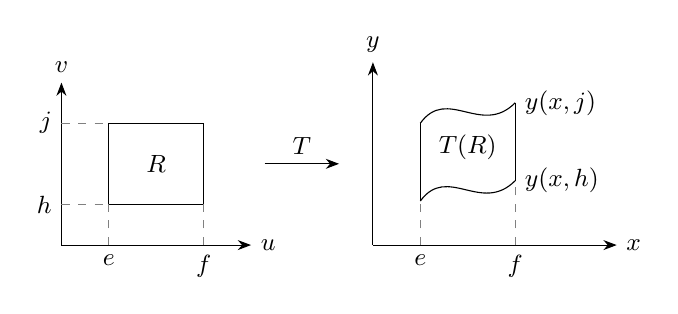
\begin{tikzpicture}[>=Stealth,font=\small,scale=.86]
  \draw[->] (0,0)--(2.8,0) node[right] {$u$};
  \draw[->] (0,0)--(0,2.4) node[above] {$v$};
  \draw (.7,.6) rectangle (2.1,1.8);
  \node[below] at (.7,0) {$e$};
  \node[below] at (2.1,0) {$f$};
  \node[left] at (0,.6) {$h$};
  \node[left] at (0,1.8) {$j$};
  \draw[dashed,gray] (.7,0)--(.7,.6) (2.1,0)--(2.1,.6)
    (0,.6)--(.7,.6) (0,1.8)--(.7,1.8);
  \node at (1.4,1.2) {$R$};
  \draw[->] (3,1.2)--(4.1,1.2) node[midway,above] {$T$};
  \begin{scope}[shift={(4.6,0)}]
    \draw[->] (0,0)--(3.6,0) node[right] {$x$};
    \draw[->] (0,0)--(0,2.7) node[above] {$y$};
    \draw (.7,.65) .. controls (1.1,1.2) and (1.6,.45) .. (2.1,.95);
    \draw (.7,1.8) .. controls (1.1,2.35) and (1.6,1.6) .. (2.1,2.1);
    \draw (.7,.65)--(.7,1.8) (2.1,.95)--(2.1,2.1);
    \draw[dashed,gray] (.7,0)--(.7,.65) (2.1,0)--(2.1,.95);
    \node[below] at (.7,0) {$e$};
    \node[below] at (2.1,0) {$f$};
    \node[right] at (2.1,.95) {$y(x,h)$};
    \node[right] at (2.1,2.1) {$y(x,j)$};
    \node at (1.4,1.45) {$T(R)$};
  \end{scope}
\end{tikzpicture}

\end{document}